% -*- TeX-engine: default; -*-
\documentclass[10pt,sigconf]{acmart}
\usepackage[font=footnotesize]{subcaption}
\usepackage[utf8]{inputenc}
\usepackage[T1]{fontenc}
\usepackage{url}
\usepackage{booktabs}
\usepackage{xcolor}
\usepackage{enumitem}
\usepackage{algorithm}
\usepackage[noend]{algpseudocode}

\setcopyright{rightsretained}
\acmYear{2018}
\copyrightyear{2018}
\acmConference[CoNEXT'18]{ACM CoNEXT 2018}{December 2018}{Heraklion/Crete, Greece}

\begin{document}
\title{The eXpress Data Path: Programmable Packet Processing for the Linux Kernel}
\author{Toke Høiland-Jørgensen}
\affiliation{%
  \institution{Karlstad University}}
\email{toke.hoiland-jorgensen@kau.se}

\author{Jesper Dangaard Brouer}
\affiliation{%
  \institution{Red Hat}}
\email{brouer@redhat.com}

\author{Daniel Borkmann}
\affiliation{%
  \institution{Cilium.io}}
\email{daniel@iogearbox.net}

\author{John Fastabend}
\affiliation{%
  \institution{Cilium.io}}
\email{john@cilium.io}

\author{David Ahern}
\affiliation{%
  \institution{Cumulus Networks}}
\email{dsahern@gmail.com}

\author{David Miller}
\affiliation{%
  \institution{Red Hat}}
\email{davem@redhat.com}

\renewcommand{\shortauthors}{T. Høiland-Jørgensen et al.}
\renewcommand{\shorttitle}{The eXpress Data Path}
\captionsetup{font+=small}



\begin{abstract}
  Programmable packet processing in software has become increasingly popular, as
  increases in computational power has made it possible to run custom
  programmable pipelines at high speeds. Often, this is implemented by so-called
  kernel bypass techniques, where a userspace application takes complete control
  of the networking hardware to avoid expensive context switches between kernel
  and user space. However, this approach makes high-speed packet processing an
  all-or-nothing proposition, where the processing application has to either
  handle all network traffic itself, or perform cumbersome re-injection of
  packets into the kernel.

  In this paper, we present an alternative approach to programmable packet
  processing, where the kernel provides a safe execution environment for custom
  packet processing applications, executed in the context of the kernel device
  driver. This system, called the eXpress Data Path (XDP), is part of the
  mainline Linux kernel, and has been gradually expanded over the last several
  releases. We show that XDP achieves a maximum packet processing performance of
  25 million packets per second on a single core, and illustrate the flexibility
  of the programming model through three example use cases: inline DDOS
  protection, layer-3 routing and layer-4 load balancing.
\end{abstract}

% TODO: Add ccsxml tags and update keywords

\keywords{XDP, Programmable Networking}
\maketitle

\section{Introduction}%
\label{sec:introduction}
High-performance packet processing in software has very tight bounds on the time
spent processing each packet ($\simeq6$~ns per packet at 100 Gbps). Network
stacks in general purpose operating systems typically perform too many
operations per packet to be able to keep up with this packet rate, which has led
to increased popularity of special-purpose toolkits for software packet
processing, such as the Data Plane Development Kit (DPDK)~\cite{dpdk}, which
bypass the operating system completely, instead passing control of the network
hardware directly to the network application. This approach can significantly
improve performance, but has the drawback that it is more difficult to integrate
with the existing networking stack, and applications have to re-implement large
parts of the stack. In the worst case, this leads to the need to operate two
separate stacks; one to perform high-speed packet processing and one to run
normal applications, leading to increased management and maintainability costs.

As an alternative to the all-or-nothing kernel bypass packet processing
technique, we present a system that adds programmability directly in the
operating system networking stack in a cooperative way, making it possible to
perform high-speed packet processing that integrates seamlessly with existing
systems, while selective leveraging functionality in the operating system. This
framework, called the eXpress Data Path (XDP), works by defining a limited
execution environment based on an extended version of the Berkeley Packet Filter
virtual machine, which allows verified programs to run directly in the device
driver context, before the kernel performs any other packet processing tasks.

XDP has been gradually integrated into the Linux kernel over the last several
releases. However, no complete architectural description of the system as a
whole exists in the literature. In this work we present such a high-level design
decription of XDP, its capabilities and how it integrates with the rest of the
Linux kernel. Our performance analysis shows raw packet processing performance
on a single core of up to 25 million packets per second. In addition,
performance scales both downwards, by decreasing CPU usage as the traffic load
drops, and upwards, by increasing performance with the number of cores dedicated
to packet processing.

Because of its integration with the kernel networking stack, and its high
performance, XDP makes it possible to implement applications that previously
required their own networking appliance, such as DDOS protection and load
balancing, directly on application servers. It also allows a hybrid approach,
where certain fast path processing is offloaded to XDP while retaining normal
network stack processing for other packets. This allows for high performance
processing without sacrificing flexibility. To illustrate these facets of XDP,
we supplement our synthetic performance benchmarks with three examples of
real-world use cases that can be implemented in XDP: inline DDOS protection on a
hypervisor host or application server; full layer-3 packet forwarding
capabilities; and layer-4 load balancing by encapsulating packets and
resubmitting them to the network.

The rest of this paper is structured as follows: Section~\ref{sec:related-work}
first outlines related work. Section~\ref{sec:design} then presents the design
of XDP and Section~\ref{sec:perf-eval} presents the raw packet processing
performance analysis. Section~\ref{sec:usecases} presents the real-world use
cases and their performance. Finally, Section~\ref{sec:limitations} presents
current limitations of XDP and future work, and Section~\ref{sec:conclusion}
concludes.

\section{Related Work}%
\label{sec:related-work}

Programmable packet processing continues to gain momentum as the performance
attainable on commodity hardware rises, and costs fall. Programmable hardware
devices such as the NetFPGA~\cite{lockwood2007netfpga}, allows this processing
to continue to happen on specialised hardware, by exposing an API that makes it
possible to run arbitrary packet processing tasks on the FPGA-based dedicated
hardware. The P4 language~\cite{bosshart2014p4} seeks to extend this
programmability to a wider variety of packet processing hardware.

However, even though specialised hardware has begun to gain data plane
programmability, the flexibility of commodity hardware has obvious advantages,
and as performance increases and cost decreases, this becomes ever more popular.
To achieve the maximum possible performance in this setting, it is necessary to
remove any bottlenecks between the networking interface card (NIC) and the
program performing the packet processing. Several systems and architectures have
been presented, that achieve this in various ways with various tradeoffs. XDP is
another such solution, with a novel approach that we believe offers a compelling
tradeoff between the various competing demands of high performance, security,
manageability and integration with existing systems. In this section we present
an overview of the previous approaches, and explain how XDP places itself in
relation to them.

Since one of the main sources of performance bottlenecks is the interface
between the operating system kernel and the userspace applications running on
top of it (because of the high overhead of a system call), most of the packet
processing frameworks are focused on managing this in various ways. This falls
into three broad categories: (a) Implementing parts of the application as a
module inside the kernel itself, (b) providing an interface for userspace to
access packet data with lower overhead than traditional socket, or (c) bypassing
the kernel entirely and handing over control of the networking device directly
to userspace.

In the first category, systems such as the OpenVswitch~\cite{openvswitch}
virtual switch and the Click~\cite{martins2014clickos} software router provide
kernel modules that offload part of their functionality into the kernel. These
are implemented as loadable kernel modules that provide configuration APIs to
userspace, but performs packet processing directly in the kernel. The drawback
to this approach is that it requires deep familiarity with internal kernel APIs,
and a failure of the network processing application in most cases leads to a
failure of the entire system.

In the second category, various systems introduce kernel modules that do not
perform packet processing themselves, but instead focus on moving packet data
out to userspace with as little overhead as possible, typically via shared
memory. Examples of this approach include PF\_RING~\cite{deri2009modern}, the
Packet I/O engine that is part of PacketShader~\cite{han2010packetshader}, and
the Netmap~\cite{rizzo2012netmap} framework.

In the third category of kernel bypass techniques, we find the PF\_RING ZC
module~\cite{pfringzc}, the hardware-specific Solarflare
OpenOnload~\cite{openonload} and, most prominently, the DataPlane Development
Kit (DPDK)~\cite{dpdk}, which started out as an Intel-specific hardware support
package, but has since seen a wide uptake under the stewardship of the Linux
Foundation.

\section{The design of XDP}
\label{sec:design}
XDP is designed to integrate with the Linux networking stack, enhancing it with
high-performance programmable hooks in strategic places. This makes it possible
to take advantage of the extensive and robust features of the operating system,
while adding custom packet processing as required. For this reason, XDP should
not be seen as a monolithic system one injects a single program into, but rather
a composition of individual parts that operate in concert to achieve the desired
outcome.

\begin{figure}[t]
\centering
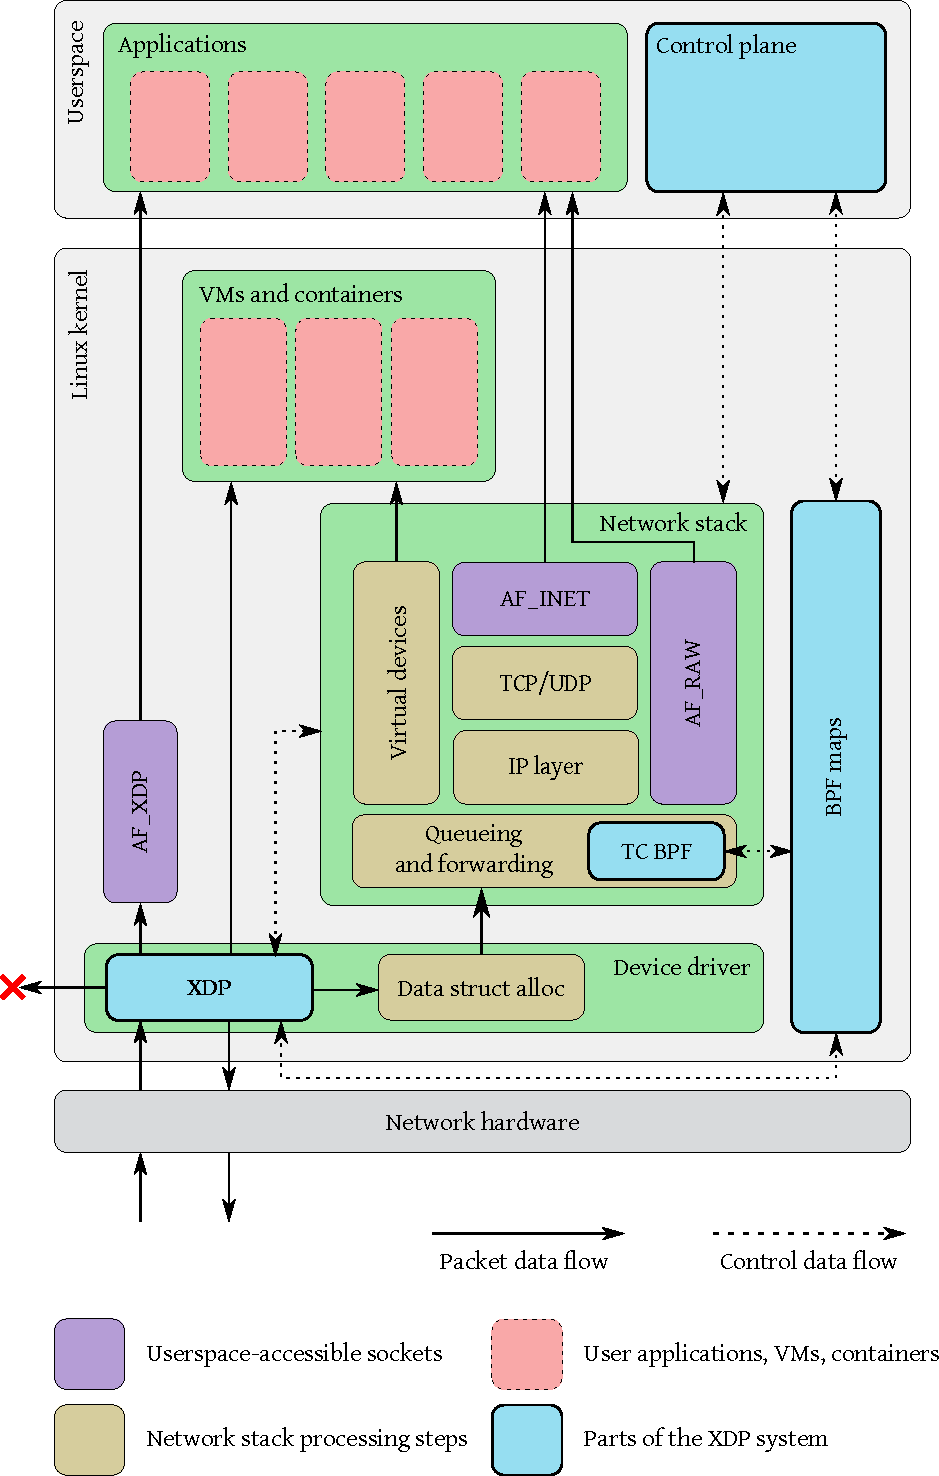
\includegraphics[width=\linewidth]{figures/kernel-diagram.pdf}
\caption{\label{fig:xdp-kernel} Diagram of how XDP integrates into the Linux
  kernel network receive path.}
\end{figure}


This section describes the various parts of the XDP system and how they fit
together. We begin with a high-level overview of the XDP programming model and
how various features of the kernel combine to form a powerful programmable data
plane. Following this, we look in detail at the extended BSD Packer Filter
(eBPF) virtual machine providing the execution model, and the in-kernel verifier
that ensures the safety of loaded eBPF programs. Finally, we give an overview of
some of the performance optimisations that are part of the XDP system, and which
help ensure high performance.

Figure~\ref{fig:xdp-kernel} shows a diagram of how XDP integrates into the Linux
kernel, and Figure~\ref{fig:xdp-execution} shows the execution flow of a typical
XDP program. Together, they give an overview of the full XDP system, and they
will be referenced throughout the exposition below.

\subsection{The XDP programming model}
\label{sec:prog-model}
The XDP system enables high-performance packet processing integrated tightly
with the rest of the Linux networking stack. This makes XDP unique compared to
other high-performance software packet processing frameworks, because it makes
it possible to selectively leverage features already implemented in Linux, while
writing custom programs to perform application-dependent processing, or to
accelerate certain parts of the data path. This section gives a conceptual
overview of the XDP programming model, explaining how the different parts fit
together.

\begin{figure*}[t]
\centering
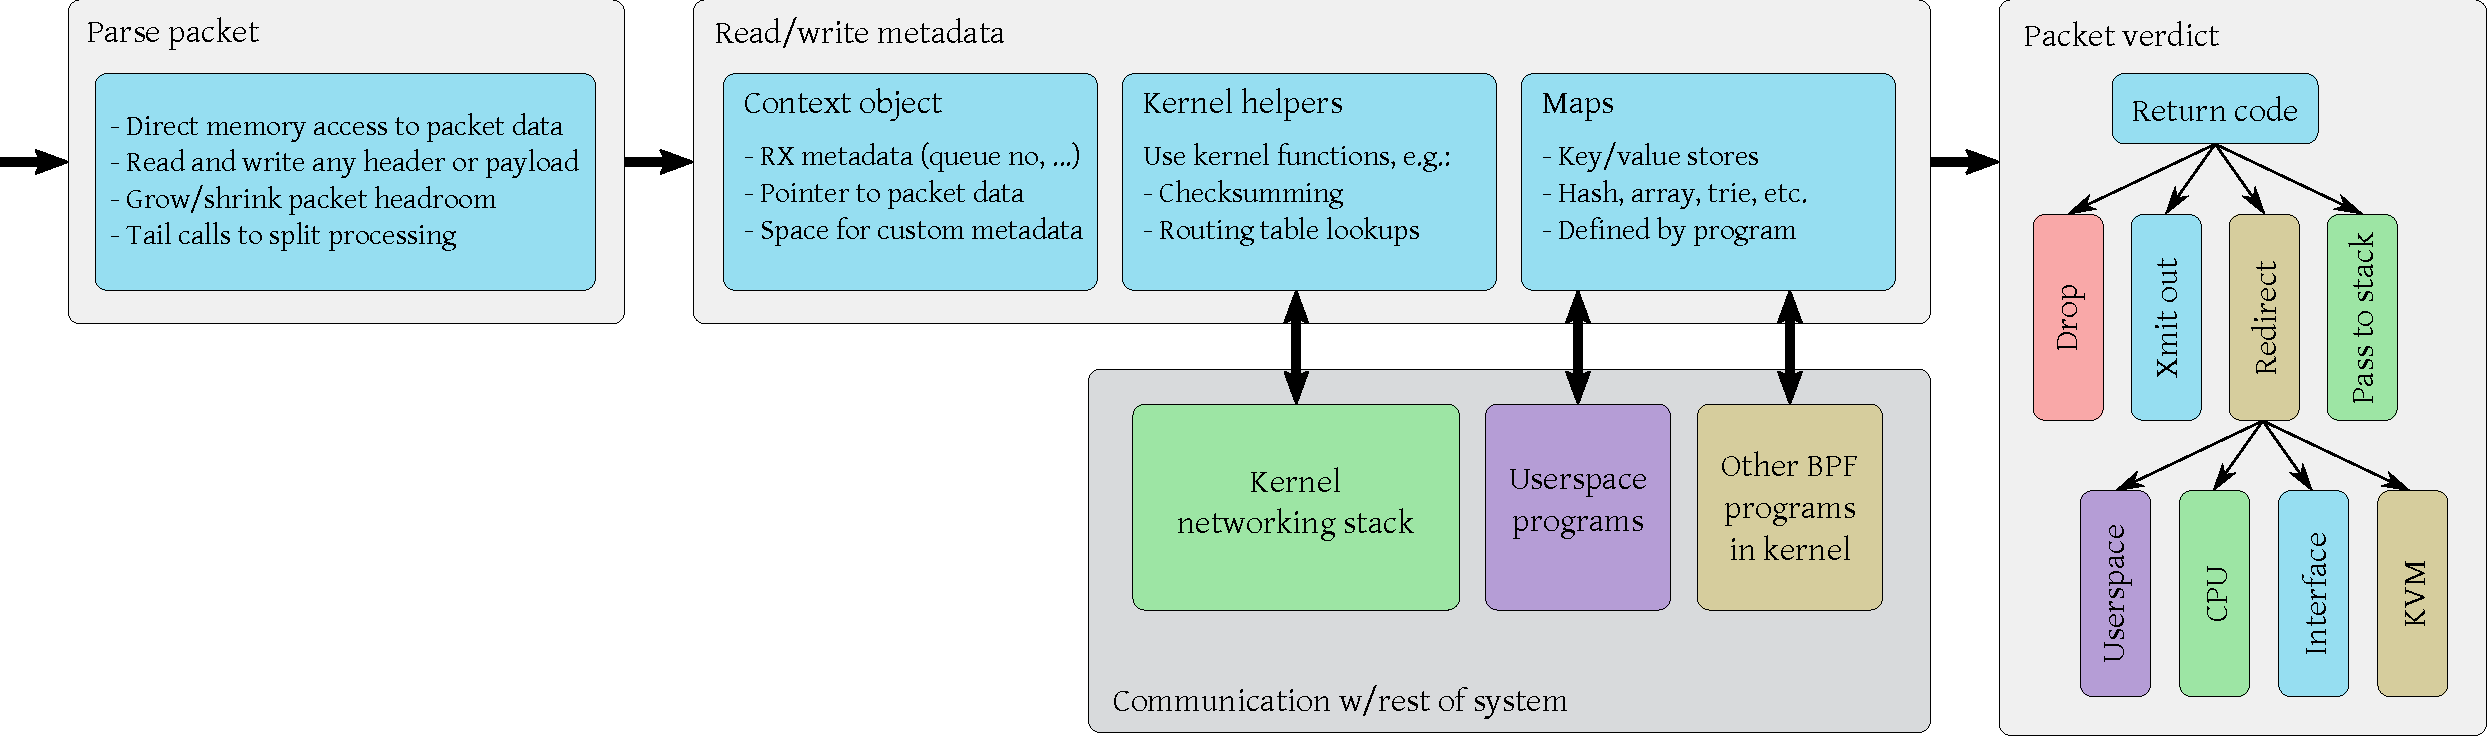
\includegraphics[width=\linewidth]{figures/xdp-execution-diagram.pdf}
\caption{\label{fig:xdp-execution} Execution diagram of a typical XDP program.
  When a packet arrives, the program starts by parsing packet headers to extract
  the information it will react on. Based on this, combined with information
  from one or more of the metadata facilities, a packet can be rewritten and a
  final verdict for the packet determined. The program can alternate between
  packet parsing, metadata lookup and rewriting, all of which are optional. The
  final verdict is given in the form of a program return code.}
\end{figure*}


An XDP program is run in the eBPF virtual machine and is entirely event driven.
The program is executed directly in context of the device driver, without
context switching to userspace. As shown in Figure~\ref{fig:xdp-kernel}, the
program is executed at the earliest possible moment after a packet is received
from the hardware, before the kernel allocates any data structures or performs
any parsing of packet data. This allows for high performance, but the program
has to parse raw packet data itself.

Figure~\ref{fig:xdp-execution} shows the various processing steps an XDP program
can perform. The program starts its execution with access to a pointer to a
context object. This object contains the buffer of the raw packet data, along
with metadata fields describing which interface and receive queue the packet
came in on, etc. The program typically begins by parsing packet data, can invoke
BPF helper functions (e.g., to perform a map lookup), or can pass control to a
different XDP program, through a so-called \emph{tail call}, which executes the
target program and never returns to the caller, thus splitting processing into
logical sub-units (based on, say, IP header version).  The context object also
contains a pointer to a special memory area is available for XDP to store
arbitrary metadata that will be available to other XDP programs, as well as to
other parts of the kernel and userspace (under certain circumstances). The
program can also write any parts of the packet data buffer, including expanding
or shrinking the packet to add or remove headers. These three steps (reading,
metadata processing, and writing packet data) correspond to the light grey boxes
on the left side of Figure~\ref{fig:xdp-execution}, and can of course alternate
and repeat in a arbitrary ways.

Similar to a regular userspace program, an XDP program ends its execution with a
return code, instructing the kernel what to do with the packet. This is shown on
the right-hand side of the figure. There are three simple return codes which
either drop the packet, immediately re-transmit it out the same network
interface, or allow the packet to be processed by the kernel networking stack.
In addition to these simple actions, the XDP program can \emph{redirect} the
packet, which controls its further processing. Redirecting can be used to
transmit the packet out a different network interface, to pass it to a different
CPU for further processing, to pass it to a virtual machine running on the host,
or to pass it directly to a special userspace socket without copying. These
different ways packets can be passed on are shown with solid lines in
Figure~\ref{fig:xdp-kernel}.

During its execution, an XDP program also has access to kernel facilities that
provide helper functions and additional metadata. These allow the XDP program to
gather additional metadata through helper functions and maps (dotted lines in
Figure~\ref{fig:xdp-kernel} and the top part of Figure~\ref{fig:xdp-execution}).
%
% I'm not sure it's 100% correct to call helper functions "callbacks"?
%
% Please correct me: AFAIK the verifier translates helper ID numbers into
% real kernel function calls (change insn->imm = bpf_func_proto->func).
% (After the verifier have checked that R1-R5 argument passing registers
% are correct and compliant).
% (based on reading kernel/bpf/verifier.c function call fixup_bpf_calls
%
% I'm not sure if the CPU still sees this as an indirect-function pointer call,
% when JIT translated?
%
Helper functions are callbacks implemented in the kernel that an XDP program can
call to make use of kernel functionality in its processing. These helpers range
serve various purposes, ranging from simple checksum computation and hashing, to
full access to the kernel routing table. New helpers are actively been added by
the kernel development community in response to user requests, continuously
expanding the functionality that XDP programs can make use of.

Maps are key/value stores that are defined by the user before loading an XDP
program, and can be referred to from within the eBPF code. Maps are shared, both
between different eBPF programs running at various places in the kernel, as well
as between eBPF and userspace. The map types include generic hash maps, arrays
and radix trees, as well as specialised types containing pointers to eBPF
programs, or even recursive pointers to other maps. Maps serve several purposes:
they are a persistent data store between invocations of the same eBPF program; a
global coordination tool, where eBPF programs in one part of the kernel can
update state that changes the behaviour in another; and a communication
mechanism between userspace programs and the kernel eBPF programs, similar to
the communication between control plane and data plane in other programmable
package processing frameworks.

Another piece of the XDP picture is the ability to run eBPF programs in other
parts of the kernel. These include packet processing in the Traffic Control (TC)
subsystem, where eBPF programs can filter packets after they have been parsed by
the kernel, or before they are passed to the hardware from applications. This is
marked as ``TC BPF'' in Figure~\ref{fig:xdp-kernel}. In addition, eBPF programs
can be attached to various places in the kernel that are unrelated to networking
(not shown in the figures). These include \emph{cgroups}, which control resource
usage for groups of processes (used for implementing containers on Linux, for
instance), as well the \emph{tracepoint} and \emph{kprobe} introspection
subsystems which allow attaching eBPF programs to arbitrary kernel functions.
Because all eBPF programs can share the same set of maps, this makes it possible
for XDP programs to react to arbitrary events in the kernel, for instance by
dropping packets if processing load increases. Because of this integration, the
XDP programming model is considerably more powerful than just the XDP programs
itself.

A final important feature of the XDP system is the ability to dynamically load
eBPF programs. Because the kernel manages the life cycle of all eBPF programs,
they can be dynamically loaded and reloaded at runtime. Combined with dynamic
dispatch to other programs using tail calls, this makes it possible to limit the
amount of processing actually performed on packets. A processing pipeline can
simply split its processing into separate XDP programs and dynamically load and
unload them as features are enabled or disabled through control plane
configuration. This also makes it possible to dynamically compile programs with
hard-coded values derived from configuration, avoiding expensive data structure
lookups for common tasks.

The various pieces of the XDP system outlined above combine to form a powerful
programmable data plane, with integration into the Linux kernel aiding
deployment on existing systems. The following sections describe the eBPF virtual
machine itself, and the verifier that ensures that loaded programs are safe to
run in kernel space.

\subsection{The eBPF virtual machine}
\label{sec:bpf-vm}
The eBPF virtual machine is an evolution of the original BSD packet filter (BPF)
\cite{mccanne_bsd_1993} which has seen extensive use in various packet filtering
applications over the last decades. BPF uses a register-based virtual machine to
describe filtering actions. This virtual machine has two 32-bit registers and
understands 22 different instructions. This makes BPF well-suited for packet
filtering operations, but limited as a general purpose virtual machine. eBPF
extends the original BPF virtual machine to allow full general purpose execution
and efficient just-in-time (JIT) compilation into native machine code. Support
for compiling (restricted) C code into eBPF is included in the LLVM compiler
suite

The code running in the virtual machine is executed directly in the kernel
address space, which makes eBPF useful for a wide variety of tasks in the Linux
kernel. The verifier (described in the next section) ensures that user-supplied
programs cannot harm the running kernel, which enables a wide array of
integrations between the running kernel and the XDP system.

The eBPF modifies the BPF virtual machine as follows:

\begin{table}[tbp]
\caption{\label{tbl:reg-map}
eBPF to x86\_64 register mapping.}
\centering
\begin{tabular}{ll|ll|ll}
\toprule
eBPF & x86\_64 & eBPF & x86\_64 & eBPF & x86\_64\\
\midrule
R0 & rax & R4 & rcx & R8 & r14\\
R1 & rdi & R5 & r8 &  R9 & r15\\
R2 & rsi & R6 & rbx & R10 & rbp\\
R3 & rdx & R7 & r13\\
\bottomrule
\end{tabular}
\end{table}


\begin{itemize}
\item The number of registers is increased to eleven, and register widths are
increased to 64 bits, with 32-bit sub-registers accessible through certain
instructions to provide compatibility with classic BPF programs. The 64-bit
registers map one-to-one to hardware registers on all 64-bit architectures
supported by the kernel, which eases JIT compilation. For instance, the x86\_64
JIT compiler uses the mapping shown in Table \ref{tbl:reg-map}.

\item eBPF adds a \emph{call} instruction for function calls, and adopts the same calling
convention as the C language conventions used on the architectures supported
by the kernel. Along with the register mapping mentioned above, this makes it
possible to map a BPF call instruction to a single native call instruction,
enabling function calls to native kernel functions with close to zero
overhead. This facility is used by eBPF to support helpers that eBPF programs
can call to interact with the kernel while processing.

The eBPF calling convention is as follows:
\begin{itemize}
\item \texttt{R0} contains the function return value
\item \texttt{R1}-\texttt{R5} contains function arguments
\item \texttt{R6}-\texttt{R9} are callee saved registers that will be preserved across the call
\item \texttt{R10} is a read-only frame pointer to the beginning of the eBPF stack space
\end{itemize}
\end{itemize}


A BPF program starts its execution with \texttt{R1} containing a pointer to a \emph{context}
object, the contents of which varies with the type of program. For XDP, this
points to a structure that allows the BPF program to access the packet data
itself, as well as various items of metadata, including space for arbitrary data
that is carried along with the packet and is accessible by other BPF programs
that operate on the packet at later stages of processing.


\subsection{The eBPF program verifier}
\label{sec:bpf-verifier}
As mentioned in the previous section, eBPF code runs directly in the kernel
address space, which means that it theoretically has full access to the running
kernel and can either crash or compromise this. To avoid this unpleasant
situation, the kernel enforces a single entry point for loading all BPF programs
(through the \texttt{bpf()} system call). When loading a BPF program it is first
analysed by the in-kernel \emph{BPF verifier}, which ensures that the program
performs no actions that are unsafe (such as reading arbitrary memory), and that
the program will terminate by disallowing loops and limiting the maximum program
size. The verifier works by first building a directed acyclic graph (DAG) of the
control flow of the program. This DAG is then verified as follows:

\begin{table}[tbp]
\caption{\label{tbl:vrf-state-vars}
eBPF verifier state variables}
\centering
\begin{tabular}{ll}
\toprule
Variable & Contains\\
\midrule
\texttt{type} & One of the types in Table \ref{tbl:reg-types}\\
\texttt{id} & ID for tracking copies of same variable\\
\texttt{fixed\_offset} & Pointer offset (after arithmetic)\\
\texttt{range\_unsigned} & Min and max values (unsigned)\\
\texttt{range\_signed} & Min and max values (signed)\\
\texttt{tnum} & Mask and value of known bits\\
\bottomrule
\end{tabular}
\end{table}

First, the verifier performs a depth-first search on the DAG to ensure it
contains no loops (no backwards jumps) and that it contains no unsupported or
unreachable instructions. Then, in a second pass, the verifier walks all
possible paths of the DAG while tracking the state of all registers. The purpose
of this second pass is to ensure that the program performs only safe memory
accesses, and that any helper functions are called with the right argument
types. This is ensured by rejecting programs that perform load or call
instructions with invalid arguments. Argument validity is determined by tracking
the state of all registers and stack variables through the execution of the
program, as explained in the following.

\subsubsection{Register state tracking}
\label{sec:reg-state}
To track data access, the verifier assigns five state variables to each
register, listed in Table \ref{tbl:vrf-state-vars}, with the possible types listed in
Table \ref{tbl:reg-types}. The fixed offset is used to track the result of pointer
arithmetic with fixed values, while the ranges and \emph{tnum} are used to track
variable offsets of pointers, as well as the ranges of scalar variables.

\begin{table}[tbp]
\caption{\label{tbl:reg-types}
eBPF verifier type annotations. The last column indicates whether pointer arithmetic is allowed for this type of pointer.}
\centering
\begin{tabular}{lll}
\toprule
\multicolumn{3}{c}{\textbf{Non-pointer types}} \\
Name & Meaning \\
\midrule
\texttt{NOT\_INIT}            & Not initialised         \\
\texttt{SCALAR\_VALUE}        & Any numerical value       \\
\midrule
\multicolumn{3}{c}{\textbf{Pointer types}} \\
Name & Pointing to & Arithm\\
\midrule
\texttt{CTX}                  & Context              & Yes \\
\texttt{MAP}                  & BPF map              & No  \\
\texttt{MAP\_VALUE}           & Value in map         & Yes \\
\texttt{MAP\_VALUE\_OR\_NULL} & Value in map or NULL & No  \\
\texttt{STACK}                & Stack frame          & Yes \\
\texttt{PACKET}               & Packet data start    & Yes \\
\texttt{PACKET\_END}          & Packet data end      & No  \\
\bottomrule
\end{tabular}
\end{table}

At the beginning of the program, \texttt{R1} contains a pointer to the execution
context, and its type is a \texttt{CTX} pointer; \texttt{R10} is a \texttt{STACK}
pointer, and all other registers are \texttt{NOT\_INIT}. At each execution step,
register states are updated based on the operations performed by the program.
When a new value is stored to a register, it inherits the state variables of the
source of the value. Arithmetic operations on scalar values will affect the
value of the \emph{tnum} state variable, which tracks which bits in a register
are known, and their value. The \emph{tnum} is a pair of \emph{mask}, which
contains the bits whose value is unknown, and a \emph{value} which contains the
bits that are known to be set to 1. Load operations set these, for instance
loading a byte from memory will result in the top 56 bits being known to be
zero, and the bottom 8 bits to be unknown. Arithmetic updates these values
according to their operation.

Branches in the instruction tree will update the register state according to the
logical operation contained in the branch. For example, a comparison "\texttt{R1
  > 10}" compare will set the maximum value of \texttt{R1} to 10 in one branch,
and the minimum value to 11 in the other. If a comparison is performed with a
scalar value rather than a constant, the knowledge of which bits are set is used
to compute the ranges for the branches (using the minimum and maximum possible
values of unknown bits as appropriate). Finally, a branch that checks whether
register with a \texttt{MAP\_VALUE\_OR\_NULL} pointer is different from
\texttt{NULL} will turn that register into a pointer with type
\texttt{MAP\_VALUE} in the \emph{true} branch, which makes it possible to
derefence the pointer.

Using the information contained in the state variables, it is possible for the
verifier to predict the ranges of memory that it is possible for each load
instruction to access. It uses this information to ensure that only safe memory
accesses are performed. For pointers to context objects, the execution context
of the eBPF program indicates allowed memory offsets for their context objects
through a callback performed by the verifier. For map values, the map definition
defines the size of the values, which is used to bound the allowed memory
accesses. For pointers to stack values, only ranges previously stored on the
stack are valid. And finally, for pointers to packet data, only ranges known to
be less than the packet length (by appropriate compares against the packet end
pointer) are allowed. Any eBPF program that makes memory accesses that the
verifier cannot prove are safe are simply rejected at load time. The verifier
also uses the range information to enforce aligned memory accesses.

When pointers are copied to other registers, a bounds check on one copy can be
used to infer the valid ranges of the other copies, even after the copy
occurred. The \emph{id} state variable is used for this purpose for packet access and
map value pointers. For packet access, all pointers with the same variable
range will have the same \emph{id}, even if their fixed offset differs. Thus, a range
check on one copy will mark the same range (minus any differences in fixed
offsets) as valid in the other copies. Similarly, for pointers to map values,
all copies of a pointer returned from the same map lookup share their \emph{id}, and
a check against NULL will be valid for all of them.



\subsection{Performance Optimisations in XDP}
\label{sec:perf-optim-xdp}

Much of the performance improvement that XDP represents over the standard Linux
networking stack is due to the processing happening before data structures are
created and memory allocated. However, there are also a couple of performance
enhancement techniques that have specifically been applied over the development
of XDP (although some of them also benefit the normal stack). In this section we
outline these techniques, and how they apply to XDP.

Packet processing on general-purpose hardware, as is done with XDP, inevitably
carries some overhead costs related to getting the packets transferred to the
system memory, processing them by the CPU, and sending them back to the
hardware. Amortising these costs over multiple packets through bulking is an
essential technique to achieve high performance. In Linux, there are two main
ways bulking is achieved: On the receive path, the NAPI mechanism~\cite{napi}
amortises the cost of interrupts from the hardware, by temporarily turning off
interrupts each time a packet is received, and instead polling to receive a
batch of packets at once. This mechanism has been available in Linux for a long
time; but for XDP it carries with it additional benefits, since the XDP program
can be executed directly in the NAPI poll context.

A similar issue is seen on the transmit path, where updating the tail pointer in
the device ring buffer initiates a transmit operation to the hardware, which
carries with it some overhead. To amortise this, XDP uses two mechanisms: When
the XDP program indicates that the packet should be transmitted out on the same
interface it came in on, it is put into the transmit ring buffer immediately,
but the tail pointer update is deferred until the end of the NAPI poll sequence,
which causes batching of all packets in the same sequence on transmit as well.
When redirecting packets to a different interface, another mechanism is used to
achieve the same thing: the redirect mechanism can use a BPF map to lookup the
destination interface. When doing so, the map also contains a buffer that will
be used to batch packets from subsequent calls, and defer the actual
transmission out of the destination interface until the end of the NAPI poll
sequence. Using the map structure to achieve this makes it transparent to the
calling program and even the device driver.

\textbf{FIXME: Is the above correct? And is there anything else we need to add
  to this section?}

\section{Performance evaluation}
\label{sec:perf-eval}
In this section we present our performance evaluation of XDP, using synthetic
benchmarks to look at specific aspects of the packet processing capabilities. In
the next section, we supplement this with a description and evaluation of a
series of real-world use cases.

For all benchmarks, we use a machine equipped with a hexa-core Intel Xeon
E5-1650 v4 CPU running at 3.60GHz, equipped with two Mellanox ConnectX-5 Ex VPI
dual-port 100Gbps network adapters. We use the TRex packet
generator~\cite{cisco18:_trex_traff_gener} to produce the test traffic. The test
machine runs a version of the Linux kernel that will be released as v4.18. The
needed XDP redirect changes to NIC driver mlx5 is expected to appear in v4.19.

% Jesper have a git tree (branch xdp_paper01) that we use for testing here:
%  https://git.kernel.org/pub/scm/linux/kernel/git/hawk/net-next-xdp.git/

To show the performance achievable with XDP, we perform the following
measurements, which correspond to the four different return codes shown in
Figure~\ref{fig:xdp-execution} above:

\begin{itemize}
\item Packet drop performance. We install a simple XDP program that drops
  packets immediately after receiving them, to examine the maximum possible
  packet processing performance.

\item Packet mirroring performance. Here we measure the performance of sending
  packets out the same network interface that they arrived on.

\item Packet forwarding performance. Here we install a simple XDP program that
  redirects packets out a different interface as they arrive.

\item Inline packet processing. We install an XDP program that allows the
  packets to proceed to the kernel networking stack, to measure the overhead
  that XDP processing introduces in the kernel receive path.
\end{itemize}


For all of these tests, we measure the maximum how many packets per second the
system can process, by running the packet generator at line speed and measuring
how many packets are processed by the test machine (the rest are simply dropped
by the hardware). We compare the performance with the \texttt{testpmd} example
application shipped with DPDK framework, and with the regular Linux kernel
network stack. For all tests, we use minimum-sized (64 bytes) packets, since
processing a high number of packets per second is the most challenging.

\subsection{Performance Tuning}
\label{sec:performance-tuning}

As we will see in the results below, our tests push the hardware to its very
limits. As such, tuning the performance of the system as a whole is important to
realise optimal performance. This section outlines some important areas where
this is needed for our experiments. In addition, we make the full details of our
setup, links to source code and the raw test data available in an online
repository~\cite{test-data}, to help others reproduce our results.

To ensure optimal performance, care needs to be taken when selecting the
hardware to run on: Our test machine has memory modules installed in all four
memory slots, to get the full available memory bandwidth. In addition, the CPU
supports Intel's Data Direct I/O (DDIO) technology, which makes it possible for
the networking hardware using Direct Memory Access (DMA) to place data directly
into the processor cache. This eliminates cache misses on subsequent processing
of the data, which is important for performance. Finally, we also make sure to
install the network card in a 16-lane PCI Express v3 slot, as smaller slots do
not provide enough bandwidth.

On the software side, a few configuration settings in the Linux kernel build are
important to mention. The first one is that we disable the ``retpoline''
mitigation for the recent Meltdown and Spectre vulnerabilities, since that has a
particularly high performance cost in XDP, as it increases the cost of indirect
function calls. Work to reduce this cost in the kernel is ongoing. The second is
that we set the preemption mode to voluntary preemption, so kernel threads
cannot be forcefully interrupted. This is the default setting used by most Linux
distributions, however turning on full forced preemption is a common performance
tweak applied to the Linux kernel. In this case it hurts performance, though, so
we leave it at the voluntary setting.

There are also a few configuration settings for the network interfaces that are
important. The first one is to disable Ethernet flow control. Flow control
causes the hardware to send pause frames to the sender if its buffers are full,
in an effort to avoid packet drops. However, in our benchmarks we deliberately
overload the receiver in an effort to measure its maximum performance. Flow
control interferes with this, so we turn it off. We also tune the size of the
receive size ring buffer that is used for transmitting packets form the hardware
to the kernel. A larger buffer means that more packets can be enqueued by the
hardware, which is generally a good thing. However, if the buffer is too large,
it can cause the DDIO logic of the processor to make bad decisions: seeing a
large buffer already queued in the processor cache, it will instead move the DMA
data to the main system memory, which causes cache misses when the data is
subsequently processed, which hurts performance. Unfortunately, there is no way
to tune the DDIO mechanism itself, so we use the ring buffer size as a
workaround for this problem. Different workloads have different optimal settings
for the ring buffer size; we always use the setting that gives the highest
performance, but not what that setting is in the results sections below.

Finally, a note on how we measure the performance for different numbers of
cores: The XDP program will always run on the core that is servicing the current
packet. The network interface has a number of receive queues that can be bound
to different cores, and the hardware offers various ways to steer packets onto
different queues. We bind each receive queue to a different core, and install
steering rules into the hardware so that a range of UDP ports are mapped 1-to-1
to the different queues. This allows us to steer traffic to different CPUs are
the traffic generator, by simply dividing the traffic between the desired number
of destination ports. For DPDK, only the default hashing-based receive queue
mapping is available; however, this is sufficient, since DPDK needs to be
explicitly configured to run on a given number of cores.

\subsection{Packet Drop Performance}
\label{sec:basel-pack-proc}
Figure~\ref{fig:drop-test} shows the packet processing performance as a function
of the number of cores. The baseline performance of XDP for a single core is
26\,Mpps, while for DPDK it is 43.5\,Mpps. This scales linearly with the number
of cores, until it hits the maximum capacity of our traffic generator, at
82.5\,Mpps. DPDK reaches this with 3 cores, while for XDP it takes 4. However,
we believe it is likely that both XDP and DPDK would be able to continue scaling
beyond these limits given a suitable traffic source. \textbf{FIXME: Is this
  true?}

\begin{figure}[t]
\centering
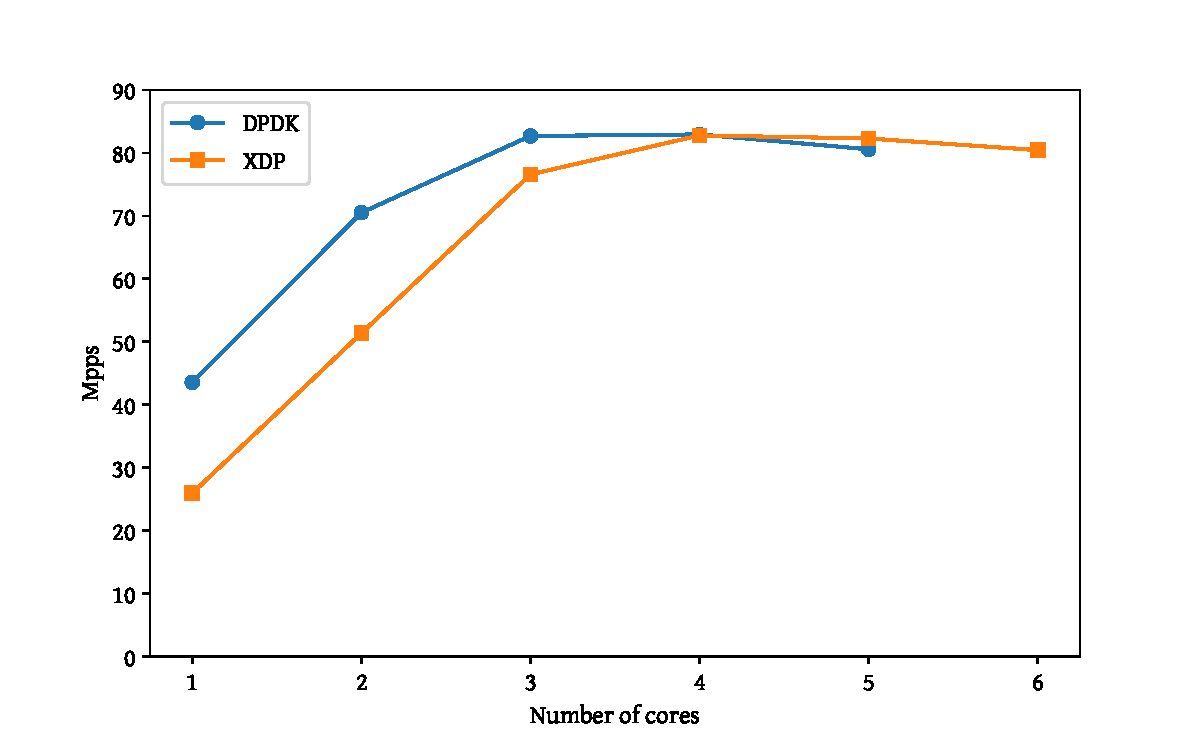
\includegraphics[width=\linewidth]{figures/drop-test.pdf}
\caption{\label{fig:drop-test} Packet drop performance. DPDK uses one core for
  control tasks, which is why it only goes to 5. The slight downward trend at
  above 4 cores is because the performance of our packet generator decreases
  when it has to generate more streams.}
\end{figure}

\begin{figure}[t]
\centering
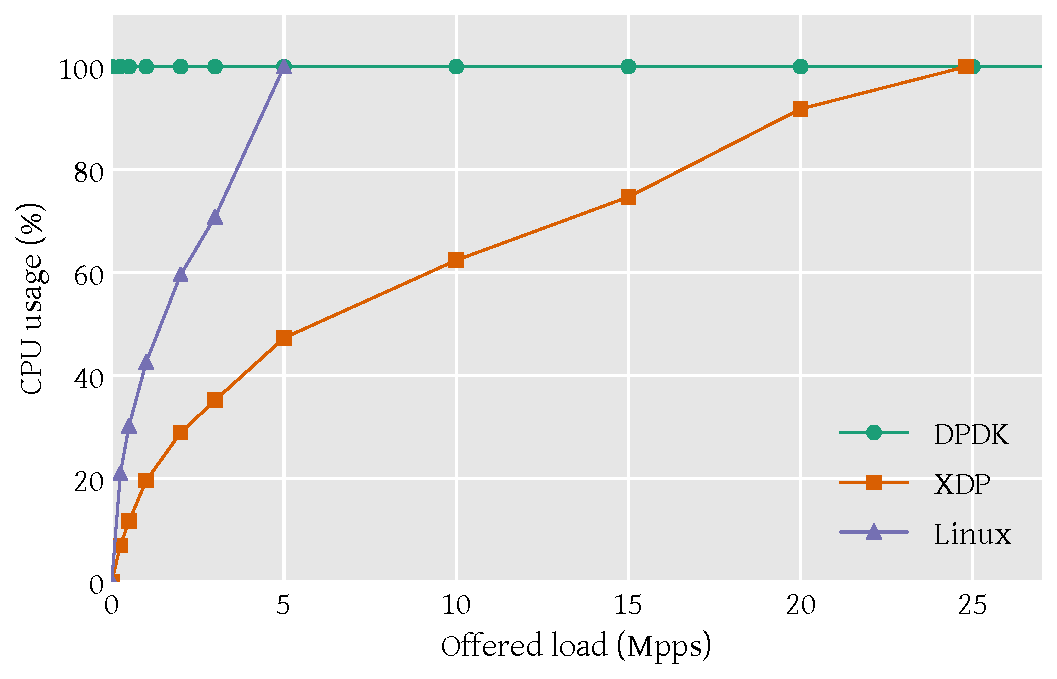
\includegraphics[width=\linewidth]{figures/drop-cpu.pdf}
\caption{\label{fig:drop-cpu} CPU usage in the drop scenario. Each line stops at
the method's maximum processing capacity.}
\end{figure}


The reason the performance dips at five and six cores is because dividing the
traffic over several cores requires using the Receive Side Scaling (RSS)
features of the hardware, which can divide up traffic between hardware receive
queues (each of which is bound to a separate core) based on packet header
information. Using this requires the traffic generator to generate the traffic
as separate flows, which means its maximum throughput drops.

\subsection{Packet Forwarding Performance}
\label{sec:pack-forw-perf}
Figure~\ref{fig:redirect-test} shows the packet forwarding performance. Again,
we see an almost linear scaling with the first couple of cores, tapering off to
sub-linear performance increases as more cores are added. We attribute this to
\textbf{FIXME}.

\textbf{FIXME: WHy the dip in DPDK performance at 2 cores? Should we re-run with
'io' forwarding mode?}


\begin{figure}[t]
\centering
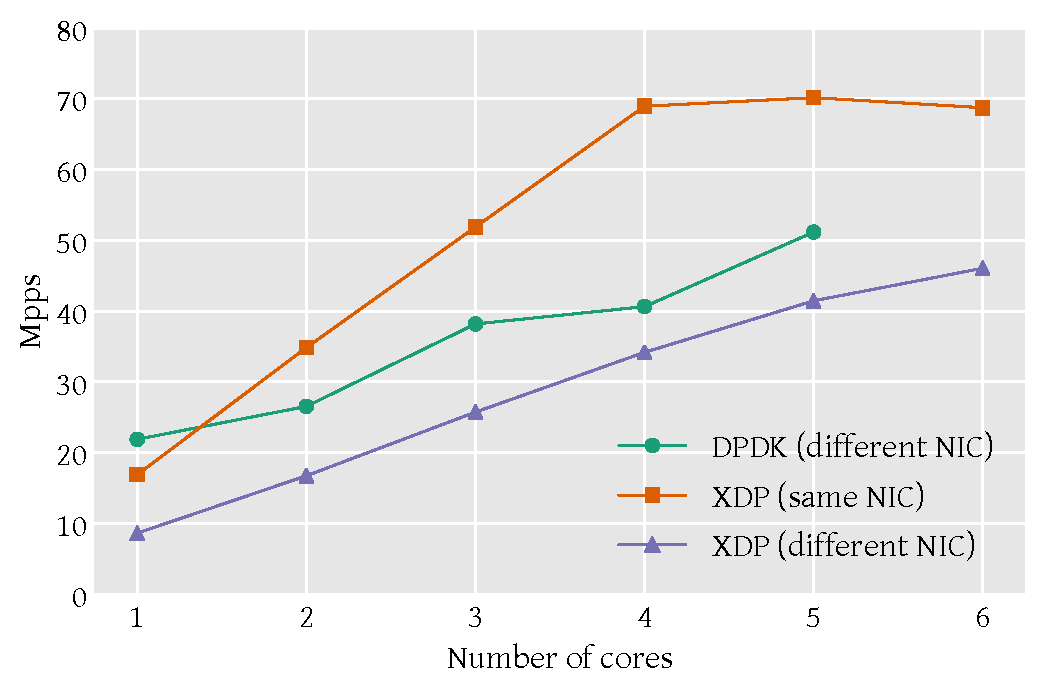
\includegraphics[width=\linewidth]{figures/redirect-test.pdf}
\caption{\label{fig:redirect-test} Packet forwarding performance.}
\end{figure}

\subsection{Packet Mirroring Performance}
\label{sec:pack-mirr-perf}
Results shown in Figure~\ref{fig:tx-test}.
\begin{figure}[t]
\centering
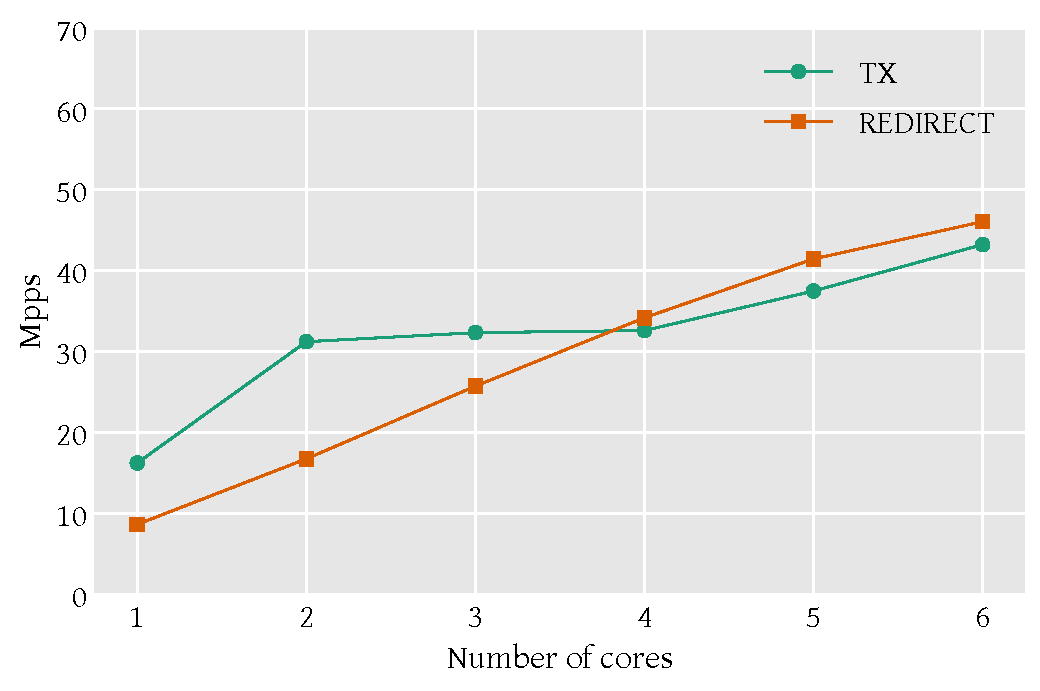
\includegraphics[width=\linewidth]{figures/tx-test.pdf}
\caption{\label{fig:tx-test} XDP\_TX vs XDP\_REDIRECT.}
\end{figure}



\subsection{Discussion}
\label{sec:perf-discussion}

% Points:
% - We do things we don't have to (e.g., DMA map/unmap)
% - We are not good enough at batching (e.g., per pkt memory return for
% redirect)
% - We cannot busy poll
%
% Absolute DROP difference XDP vs DPDK is (1/26-1/43.5)*1000 = 15.47 ns. This is
% between 55 and 145 instructions (depending on ins/cycle; perf says 2.61 for
% XDP_DROP). About 350 instructions per pkt.
% Function call overhead is 1.317 ns; mlx5 can potentially eliminate 6 of those
% for XDP_DROP - half the difference to DPDK.

\section{Real-world use cases}
\label{sec:usecases}
In this section we describe and evaluate three real-world use cases that
showcase various ways in which XDP can used to implement useful applications or
features. These use cases have all seen real-world deployment in one form or
another, although we use simplified versions in our evaluation so as to be able
to make the code available.

The three use cases are inline Denial of Service (DoS) mitigation, a software
layer-3 router, and an application load-balancer, and are described in turn in
each of the following subsections.

\subsection{Inline DoS Mitigation}
\label{sec:dos-usecase}
DoS attacks continue to plague the internet, typically in the form of
distributed attacks (DDoS attacks) from compromised devices attached to the
internet. There are various ways to mitigate them, but having some kind of
service that protects critical infrastructure is typically at least a component
of DDoS mitigation \textbf{FIXME: citation needed}. This can be done by
filtering all traffic through a device that distinguish legitimate traffic from
attacks, and drop the attack packets before they reach the application server.

The obvious problem with protecting against a DDoS attack is the sheer scale of
the traffic that needs to be dropped, which leads to the use of expensive
appliances to handle the dropping. However, with XDP we have another option:
installing the traffic filter directly on the application server in the form of
an XDP program, which is possible without any other modifications to the server.
In the case of a virtual machine deployment, the filter can even be installed on
the hypervisor, and thus protect all virtual machines running on the host.

How to identify attack traffic is not our focus here, but rather the mechanism
that drops the unwanted traffic. We simply assume that there exists \emph{some}
way of identifying which traffic is legitimate and which isn't. Because of the
dynamic nature of XDP, there are many options available: BPF maps could be used
for while-listing or black-listing, the packet payload could be inspected, etc.
It is even possible to load new XDP programs especially tailored towards
dropping a particular kind of attack traffic as the need arises. However, in our
example, we simply assume that a server hosts a TCP-based service, and so
consider all UDP traffic as unwanted.

To test the performance of such a solution, we use the Netperf benchmarking
tool~\cite{netperf}. This is equipped with a TCP-based round-trip benchmark,
which opens a TCP connection and sends a small payload which is echoed back from
the server, repeating as soon as a reply is received. The output is the number
of transactions per second, which is a good proxy for an interactive TCP
session, such as small remote procedure calls.

We first measure the baseline performance of this test, and see that we are able
to perform around 25.000 transactions per second with no competing traffic. We
then, from a separate machine, offer an increasing load of small UDP packets,
which simulates the DoS attack, and measure how the TCP application is affected.
The network interface is configured to redirect all traffic to a single receive
queue, so all packets are processed by the same CPU core. This is important in
this use case, because the machine will be running other applications on the
remaining cores, and so we don't want to dedicate too many resources to just
packet processing\footnote{The actual number of cores dedicated to packet
  processing will of course have to depend on the volume of traffic the filter
  should be able to process.}.

\begin{figure}[t]
\centering
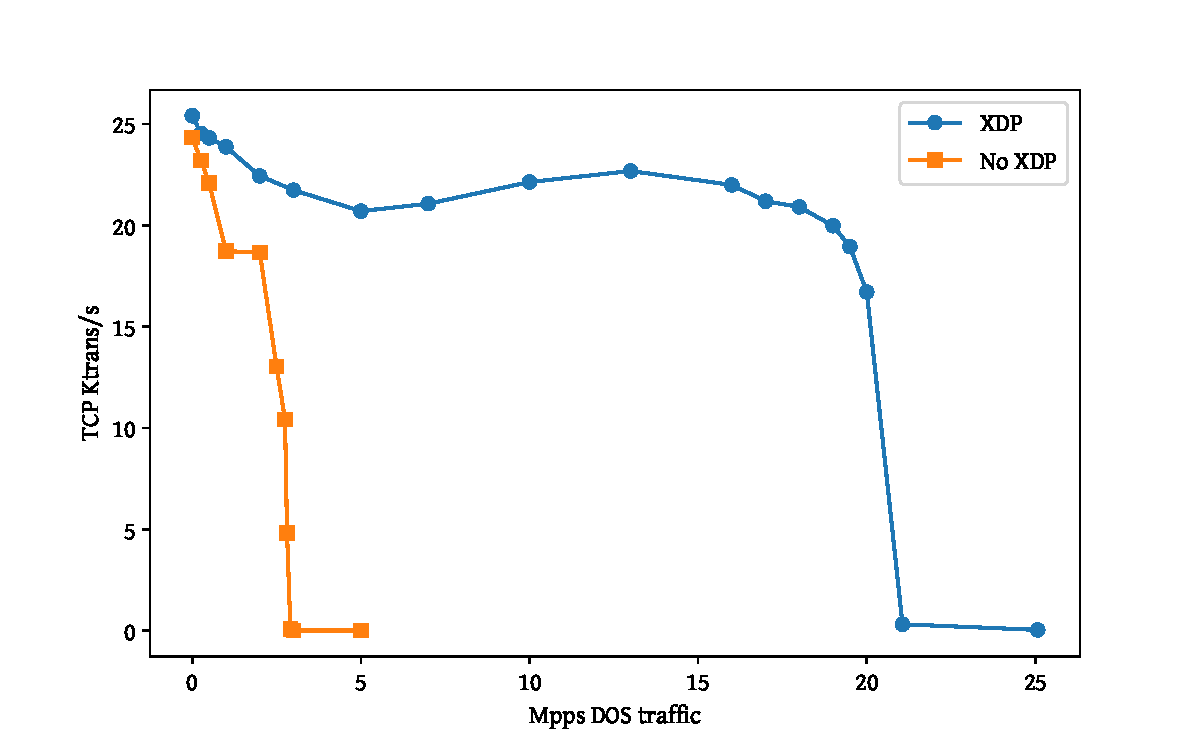
\includegraphics[width=\linewidth]{figures/ddos-test.pdf}
\caption{\label{fig:ddos-results} DDOS performance. Number of TCP transactions
  per second with different levels of UDP packet floods being sent to the
  server.}
\end{figure}

The results of this is shown in Figure~\ref{fig:ddos-results}. It is clearly
seen that without the XDP filter, performance drops significantly, being halved
at 2.5 Mpps and effectively zero at just below 3 Mpps. However, with the XDP
filter in place, performance is kept above 20.000 transactions per second up to
19 Mpps, after which it drops rapidly. The small increase in baseline
performance (from 24,500 to 25,500 transactions per second) is because the XDP
program uses the \emph{redirect} feature to move the network stack processing of
the application traffic to a separate CPU core, to make sure the application
performance is not impacted by handling of the DoS traffic.

As these results show, it is quite feasible to perform this kind of filtering in
XDP, and comfortably handle packet rates above 10\,Gbps of DoS traffic (with
minimum packet sizes) on a single CPU core. Deploying DoS mitigation this way
leads to increased flexibility, both because of the programmability offered by
XDP, but also because it eliminates the need for at separate appliance to scrub
the traffic.

\subsection{Software Router}
\label{sec:fwd-usecase}
The second use case is that of a software router. The Linux kernel already
contains a full-featured routing table, which includes support for policy
routing, source-specific routing, equal-cost multipath load balancing, and more.
And routing daemons such as Bird or FRR implement a variety of routing control
plane protocols, which makes it quite feasible to turn a Linux system into a
full-featured software router. However, thus far the data plane forwarding
performance has kept this from being feasible at very high rates.

Because of the rich ecosystem for routing on Linux, improving performance of the
kernel data plane is desirable, as re-implementing the routing stack in another
data processing framework carries a high cost. Thus, XDP is particularly suited
for this task. This is also the reason why one of the first kernel helpers
introduced to XDP is a routing table lookup function. This function makes it
possible to perform full routing table lookups directly from XDP. The result of
the lookup is an egress interface and a next-hop MAC address, which makes it
possible for the XDP program to immediately forward the packet if the lookup
succeeds. If no next-hop MAC is known (because neighbour lookup hasn't been
performed yet), the XDP program can instead pass the packet to the networking
stack, which will perform the neighbour lookup, allowing subsequent packets to
be forwarded by the XDP fast path.

To show the performance of the software router use case, we use the XDP routing
example that is included in the Linux kernel source and compare its performance
to the native Linux networking stack routing. The example simply parses the IP
header of an incoming packet, does a routing table lookup, and immediately
forwards the packet if a match is found, or passes it up to the network stack if
not. We perform two tests: one with a single route installed in the routing
table and all packets set to the same destination address. And another where we
import a full dump of the global BGP routing table from \url{routeviews.org},
where we set all next-hop addresses to the same value, but vary the destination
addresses of the packets being routed. The routing table dump contains 752,138
distinct routes, and for our tests we generate 4000 random destination IP
addresses.

The performance of this use case is seen in Figure~\ref{fig:router-fwd}.

\begin{figure}[t]
\centering
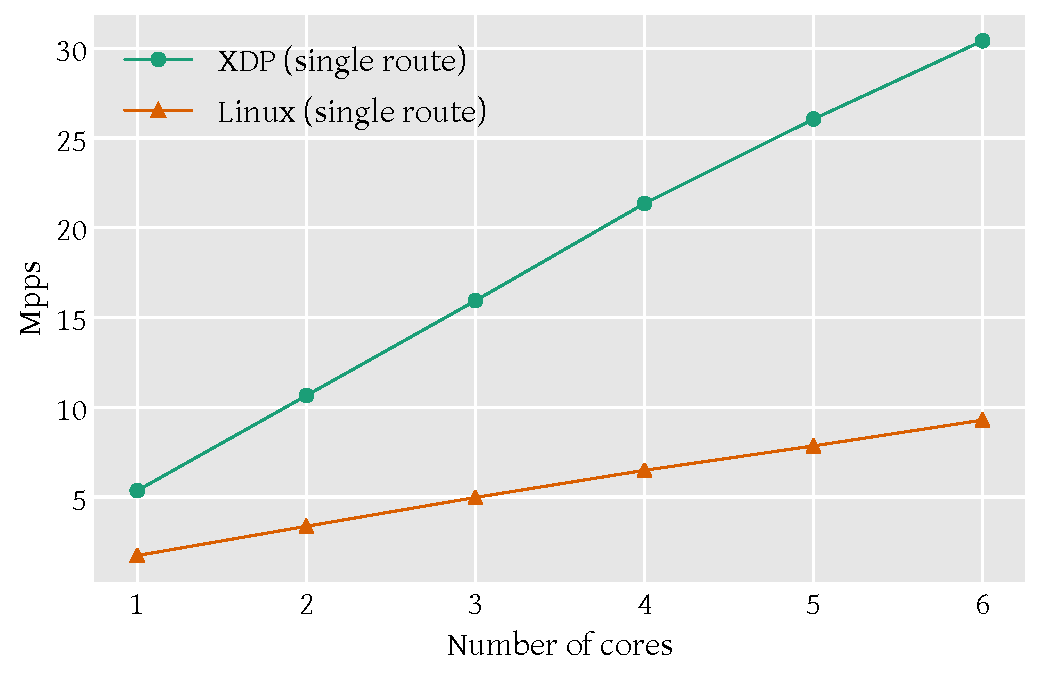
\includegraphics[width=\linewidth]{figures/router-fwd.pdf}
\caption{\label{fig:router-fwd} Software routing performance.}
\end{figure}


\subsection{Load Balancer}
\label{sec:load-balancer}
For the load balancer use case, we use the XDP component of the Katran load
balancer~\cite{katran} recently released as open source by Facebook. This works
by announcing a virtual IP address to the world, which is then routed to the
load balancer. At the load balancer, the XDP program hashes the layer-4 packet
header using a stable hashing algorithm, which becomes a destination application
server. The packet is then encapsulated in a new IP header and sent to the
application server, which is responsible for decapsulating it, processing the
request, and replying directly to the originator of the request. This means that
the XDP program can perform the packet encapsulation, and immediately return the
packet out the same interface, as in the performance test in
Section~\ref{sec:pack-mirr-perf}.

To test this use case, we configure the Katran XDP program with a fixed number
of destination hosts, and run it on our test machine. Once the packets are
returned to the network they are simply dropped; we are only interested in the
performance of the load balancer component itself. This performance is shown in
Figure~\ref{fig:load-balancer}.

\begin{figure}[t]
\centering
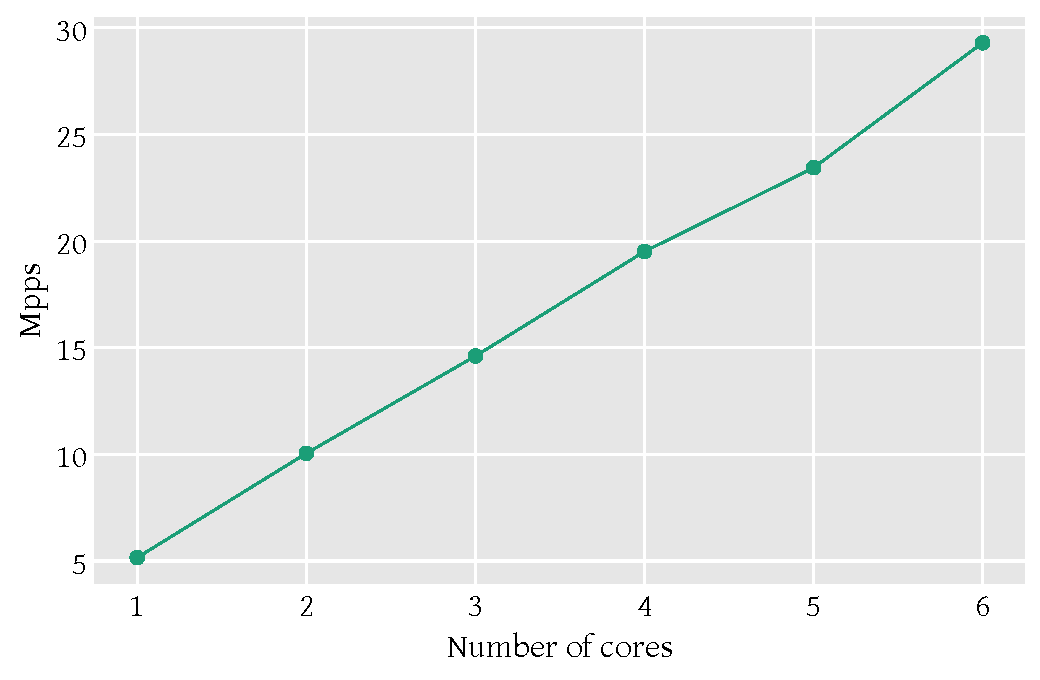
\includegraphics[width=\linewidth]{figures/load-balancer.pdf}
\caption{\label{fig:load-balancer} Load balancer performance. FIXME: This is a
  really boring graph.}
\end{figure}


\section{Limitations and future work}
\label{sec:limitations}
As we have shown above, XDP has excellent performance, and is already useful in
a variety of real-world use cases. However, XDP is also relatively new
technology that is being incrementally added to a general purpose operating
system kernel. As such, it is constantly evolving, and still has some rough
edges. In this section we present some of the known limitations, and future
directions for XDP's development. These include: User experience and debugging;
driver support; improvements to NAPI; and better handling of rate transitions.
Each of the following subsections discuss each of these issues in turn.

\textbf{FIXME: This needs to strike the right balance between ``look, we are
  improving things'' and ``there are lots of issues''. I fear it leans a bit too
far towards the latter as is, so maybe some text needs to be cut.}

\subsection{User Experience and Debugging}
\label{sec:user-exper-debugg}
Since an XDP program runs in the kernel, the debugging tools available to a
regular userspace program are not generally applicable, and even common
debugging tools such as \texttt{printf()} are unavailable. The tendency for some
operations to fail silently and just drop packets doesn't help this situation.
In addition, the subset of C that is generally used to write BPF programs can be
limiting, for instance due to the need to unroll all loops. Finally, the
verifier will sometimes reject valid programs because it cannot prove validity,
and its error messages are not always helpful. Together, these issues combine to
make writing a useful XDP application harder than it needs to be, especially for
someone not familiar with the Linux ecosystem.

Work is ongoing to improve this situation, and indeed it already has improved
some. The XDP subsystem includes a number of tracepoints, that can be accessed
by the debugging tools used for the rest of the kernel to give information about
failures of XDP actions, usage of helper functions, etc. The tools to support
this continue to improve, as does the documentation. In addition, the verifier
continuously improving to recognise more correct programs that were previously
rejected as invalid. Support for function calls in eBPF has recently been added,
and the addition of support for bounded loops is planned. However, we recognise
that this is still an area in need of improvement.

\subsection{Driver Support}
\label{sec:driver-support}
Each device driver needs to add support for running XDP programs, by supporting
an API exposed by the core networking stack. Support is continuously being added
to more and more drivers.\footnote{At the time of writing Linux 4.17 has XDP
  support in 12 different drivers, including the most popular high-speed network
  adapters. An updated list of supported drivers is included in
  \url{http://cilium.readthedocs.io/en/latest/bpf}.} However, not having
universal support is limiting and can be confusing for users. One particular
issue with this is that it is possible for drivers to support only subsets of
the XDP functionality. This is because drivers need to implement support for
each of the possible return code. This is further complicated by the fact that
support for redirection has separate implementations in the receive path and the
transmit path, so it is possible for a driver to support redirecting packets to
other interfaces, but not being the target of a redirection from elsewhere.

Ultimately, we believe that these issues will be resolved by having full support
for XDP in all device drivers. However, for obvious reasons this takes time, and
holding back the development of the system until all drivers have caught up is
not feasible. As the XDP system has evolved, the need to keep the API support
required in drivers to a minimum has become increasingly clear, and some steps
have been taken in this direction. For instance, support for new targets can be
added to the redirection action without any changes needed from the drivers.

\subsection{Improvements to NAPI}
\label{sec:improvements-napi}
As we saw in Section~\ref{sec:perf-eval}, DPDK still achieves markedly better
raw packet processing performance than XDP. The main reason for this is that the
NAPI mechanism that Linux uses to selectively switch between interrupt-based
packet processing and polling is insufficient to mitigate the large number of
interrupts that happen at high packet rates. In some cases it would be
beneficial to switch to a full busy polling mode, if one is willing to dedicate
a full CPU core to packet processing.

There have been some efforts to selective switch a network adapter to busy
polling mode, which has shown promising results~\cite{dumazet17:_busyp}. We
believe continuing this work, and integrating it with XDP, will make it possible
to reach raw packet processing performance equal to that of DPDK.

\subsection{Handling of Rate Transitions}
\label{sec:handl-rate-trans}
Currently, XDP offers no mechanism to gracefully handle rate transitions, i.e.,
cases where packets are forwarded to a destination that cannot handle the rate
of incoming packets. This can happen if, e.g., a 100\,Gbps ingress interface
attempts to forward packets to a slower 10\,Gbps interface, or to a virtual
interface or userspace application that cannot process them fast enough.

Since the XDP program signals the packet destination via its return code,
execution has already ended when the packet forwarding is attempted, and so a
failure due to a full hardware buffer or a busy userspace application cannot be
gracefully handled, and will simply result in the packet being silently dropped.
This is obviously not ideal, and exploring ways to gracefully deal with this is
planned for the future.


\section{Conclusions}
\label{sec:conclusion}
We have presented XDP, a system for safely integrating high-speed programmable
packet processing directly in the Linux kernel. This represents an alternative
solution to all-or-nothing kernel bypass solutions, which makes it easier to
integrate the packet processing with normal applications.

Our evaluation has shown that XDP achieves raw packet processing performance of
up to 25 million packets per second on a single CPU core. We have also
demonstrated three examples of real-world use cases that can be implemented with
XDP: Inline DDOS mitigation, layer-3 forwarding, and layer-4 load balancing.

XDP continues to be actively developed by the Linux community, and we believe
that it offers a compelling alternative to other high-speed packet processing
frameworks, especially where integrating with existing systems and applications
is important.

\bibliographystyle{ACM-Reference-Format}
\bibliography{xdp}

\end{document}
